\chapter{Obtenção das Bases}
\label{chapter:ObtencaoBases}
\noindent

A primeira etapa de implementação desenvolvida no trabalho foi a aquisição de um conjunto de questões rotuladas de acordo com seus assuntos para se viabilizar a aplicação de algoritmos de classificação. Esse conjunto de dados foi obtido por meio de \textit{web scrapping}. Posteriormente, os arquivos baixados foram filtrados e convertidos para um novo formato de maneira a se armazenar apenas os dados de interesse. Finalmente, desenvolveu-se uma interface que faz uso de todo esse conjunto de dados, tornando-o acessível para as demandas nos diferentes algoritmos de aprendizado de máquina. A figura \ref{fig:data_processing_pipeline} ilustra a sequência de operações executadas na aquisição de dados e que serão descritas em detalhes a seguir.

\begin{figure}[!ht]
	\centering
	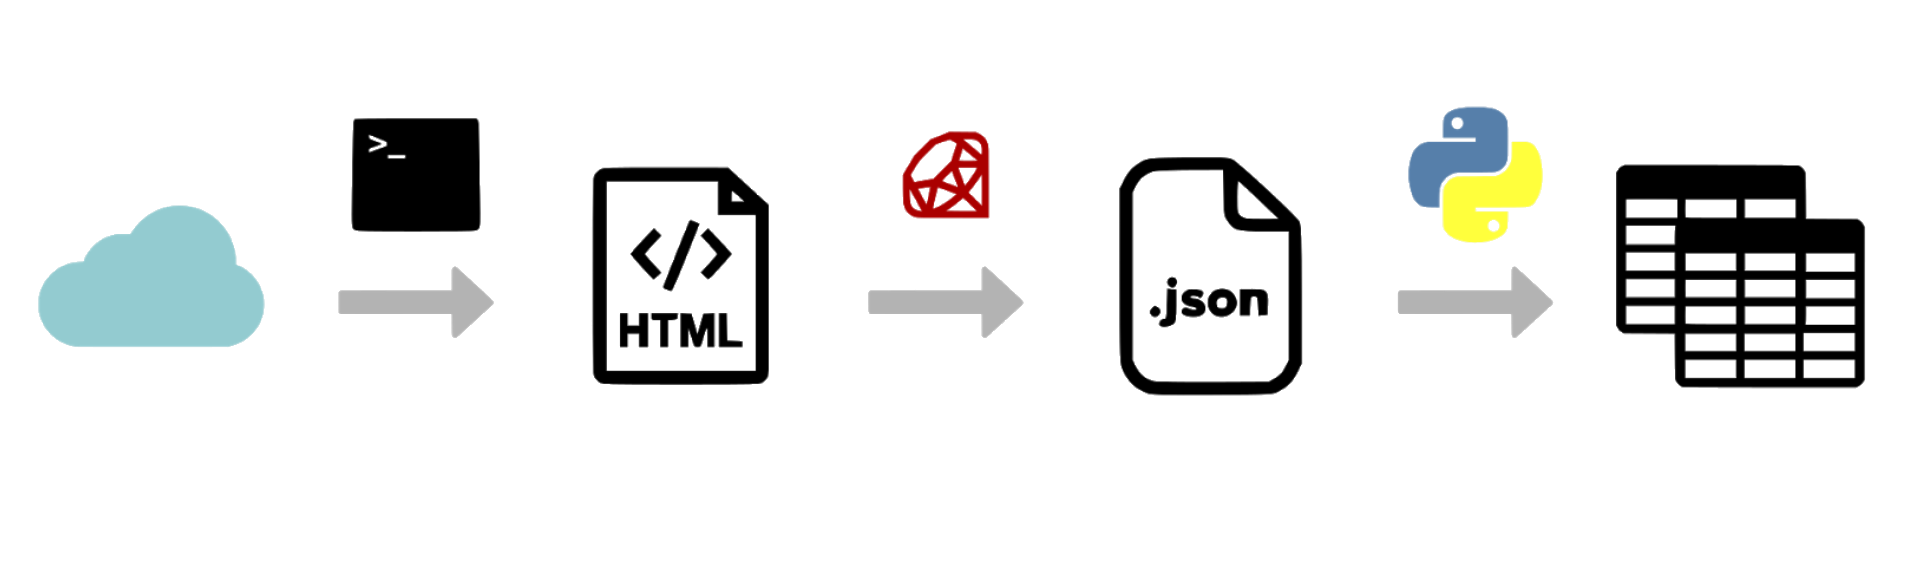
\includegraphics[width=0.9\textwidth]{figures/data_processing_pipeline.PNG}
	\caption{Sequência de operações para a aquisição de dados}
	\label{fig:data_processing_pipeline}
\end{figure}

\section{\textit{Web Scrapping}}

As questões utilizadas para treinamento dos modelos classificatórios foram retiradas de um site preparatório para concursos públicos chamado “Rota dos concursos” (rotadosconcursos.com.br). Para esta tarefa, foi implementado um \textit{script} ruby que simulava as requisições HTTP feitas por um navegador. Cada requisição realiza o \textit{download} de um arquivo HTML de uma página do site que contem exatamente uma questão de concurso público.

Devido à grande quantidade de questões, foi utilizado um serviço de servidores dedicados em nuvem para possibilitar as muitas horas de requisição. A quantidade de questões também impossibilitou a manipulação dos arquivos em um único diretório. Desta forma foi utilizado um esquema de subpastas enumeradas de 000 a 999 tornando a manipulação no sistema de arquivos tratável, pois os arquivos são uniformemente distribuídos nessas subpastas por meio de uma função de \textit{hash} simples. Além disso, como o gargalo são operações de entrada e saída (I/O \textit{bound}) nas requisições, foi utilizado \textit{multithreading} para otimizar o uso de CPU.

\section{Pré-Processamento}

Após o download em formato HTML, o conteúdo de cada página teve de ser isolado em arquivos em formato JSON. Cada arquivo continha apenas os dados referentes a uma questão, de maneira a descartar as informações referentes ao \textit{layout} da página e manter os seguintes atributos:

\begin{itemize}
\item id: Identificador único de cada questão;
\item text: Enunciado da questão;
\item subject\_path: Lista de \textit{strings} iniciada pela área de conhecimento abrangido pela questão e seguida pela hierarquia de domínios abrangidos em ordem de especificidade;
\item alternatives: Lista com o texto de cada uma das alternativas caso a questão seja de múltipla escolha;
\item image\_count: Contagem de imagens utilizadas no enunciado da questão, vale ressaltar que essa imagem pode conter até mesmo informação textual não capturada pelo atributo text;
\item concurso: Nome do concurso público do qual a questão foi extraída;
\item prova: Ano em que a prova foi aplicada;
\item banca: Banca referente ao concurso público da questão;
\item nivel: Nível de escolaridade utilizado como pré-requisito no concurso público em que questão foi obtida;
\item answer: Alternativa correspondente a resposta correta caso a questão seja de múltipla escolha.
\end{itemize}

Ao término desse pré-processamento, obteve-se um total de mais de 500 mil arquivos JSON com questões.

\section{API de dados}
\label{dataset_api}

Como uma etapa final da sequência de operações antes de se iniciar a etapa analítica, foi necessário desenvolver uma interface que fosse flexível para as diferentes demandas de dados de treinamento/validação/teste no desenvolvimento dos algoritmos de aprendizado de máquina. Para isso, foi implementada uma classe na linguagem python (mesma utilizada para na etapa seguinte) que contivesse os dados de todas as questões armazenadas inicialmente em distintos arquivos JSON em uma única estrutura de dados em memória. Para isso, utilizou-se a estrutura de um \textit{dataframe} do pacote pandas devido a sua boa performance com o uso de operações de \textit{broadcast} em um grande conjunto de dados e a sua fácil manipulação.

Além disso, foram definidos alguns parâmetros para o construtor dessa classe, de maneira a possibilitar o seu uso em diferente contextos de teste:

\begin{itemize}

  \item random\_state: Número inteiro utilizado como \textit{seed} de aleatorização quando for necessário distribuir arbitrariamente o conjunto de dados conforme é detalhado nos parâmetros \textit{frac} e \textit{subset}.
  
  \item frac: Determina a fração dos dados que vai ser carregada, possibilitando tanto um uso reduzido para maior velocidade nos testes de desenvolvimento como o uso completo para obtenção de resultados finais.
  
  \item dict\_name: Nome de um arquivo JSON utilizado como dicionário para agrupamento de assuntos. Esse parâmetro possibilita o agrupamento de assuntos similares, já que originalmente existem 133 áreas de conhecimento definidas e com grande interseção entre elas, o que inviabiliza a classificação das questões até mesmo por seres humanos especialistas, pois a classificação possuiria um caráter subjetivo. Para ilustrar a existência de domínios de conhecimento similares, pode-se citar Engenharia de Redes e Engenharia de Telecomunicações, bem como Contabilidade Privada Contabilidade Pública. Vale destacar que o fato de ser um arquivo externo usado como dicionário flexibiliza o teste de diferentes agrupamentos, permitindo a escolha de um agrupamento que resulte em uma melhor performance de classificação.
  
  \item min\_number\_per\_label: Número mínimo de amostras para cada área de conhecimento após o agrupamento, as amostras referentes a assuntos com total insuficiente são descartadas. Esse parâmetro é importante porque podem existir áreas de conhecimento com um número insuficiente de amostras para realizar o treinamento de um algoritmo de classificação.

  \item subset: Determina se o objeto a ser instanciado terá fração de dados correspondente ao treinamento, validação, teste ou todo o conjunto de dados. A divisão desses conjuntos é feita de maneira aleatória e a consistência dessa aleatorização para diferentes instâncias é determinada pelo parâmetro \textit{random\_state}.
  
\end{itemize}

Além disso, a API de dados também faz uso de cache do \textit{dataframe} base no formato de um arquivo csv para evitar a releitura das centenas de milhares de arquivos JSON sempre que for necessário criar um nova instância da classe.

Finalmente, sobre os métodos oferecidos pela API de dados, pode-se destacar a existência de métodos que retornam estruturas com dados utilizados no treinamento como o enunciado de todas as questões e seus respectivos assuntos no formato de \textit{string} ou de \textit{one-hot-encoding}. 